\immediate\write18{tex spath3.dtx}
%\immediate\write18{tex knots.dtx}
\documentclass{article}
\usepackage{tikz}
\usetikzlibrary{knots,intersections,decorations.pathreplacing}

\tikzset{
  path details/.style={
    >=stealth, 
    every node/.style={
      midway, 
      sloped, 
      font=\tiny
    },
  }
}

\begin{document}

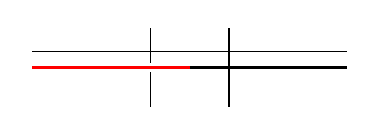
\begin{tikzpicture}
\draw (1.5,.5) -- (1.5,-.5) (2.5,.5) -- (2.5,-.5);
\draw (0,.2) -- (4,.2);
\draw[knot=red,knot gap=4,thick] (0,0) -- (2,0);
\draw[thick] (2,0) -- (4,0);
\end{tikzpicture}

\end{document}
\begin{tikzpicture}
\begin{knot}
\strand (0,0) .. controls +(1,0) and +(-1,0) .. (2,1) .. controls +(1,0) and +(-1,0) .. (4,0);
\end{knot}
\end{tikzpicture}

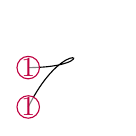
\begin{tikzpicture}
\begin{knot}[
  consider self intersections,
  draft mode=crossings,
]
\strand (0,0) .. controls +(.5,1) and +(1,0) .. (0,0.5);
\end{knot}
\end{tikzpicture}

\begin{tikzpicture}
\begin{knot}[
  consider self intersections,
  draft mode=crossings,
]
\strand (0,0) .. controls +(3,1) and +(-3,1) .. (1,0);
\end{knot}
\end{tikzpicture}


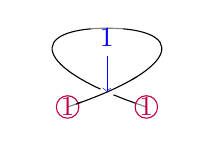
\begin{tikzpicture}
\begin{knot}[
  consider self intersections=no splits,
  draft mode=crossings,
]
\strand (0,0) .. controls +(1.5,.5) and +(1,0) .. (.5,1) .. controls +(-1,0) and +(-1.5,.5) .. (1,0);
\end{knot}
\end{tikzpicture}


\newcommand{\motif}[1]{ 
  to ++(180+#1:0.50) arc (270+#1:150+#1:0.15) 
  to ++( 60+#1:0.50) arc (-30+#1:150+#1:0.15) 
  to ++(240+#1:0.25) arc (150+#1:330+#1:0.25)
  to ++( 60+#1:0.55) arc (150+#1: 30+#1:0.20)
}
\newcommand{\celticknot}{\motif{0}\motif{120}\motif{240}}
\begin{tikzpicture}
\begin{knot}[
  line width=2pt,
  line join=round,
  clip width=2,
  clip radius=16pt,
  end tolerance=20pt,
  scale=8,
  consider self intersections,
  ignore endpoint intersections=false,
  background color=white,
  intersection 12/.style={/tikz/knot diagram/clip radius=13pt},
  every strand/.style={draw=none},
  /tikz/only when rendering/.style={
    draw=red,
    double=white,
    double distance=6pt,
    line cap=round,
  }
%  draft mode=crossings,
]
\strand (0,0) \celticknot;
\flipcrossings{1,3,6,8,10}
\end{knot}
\end{tikzpicture}

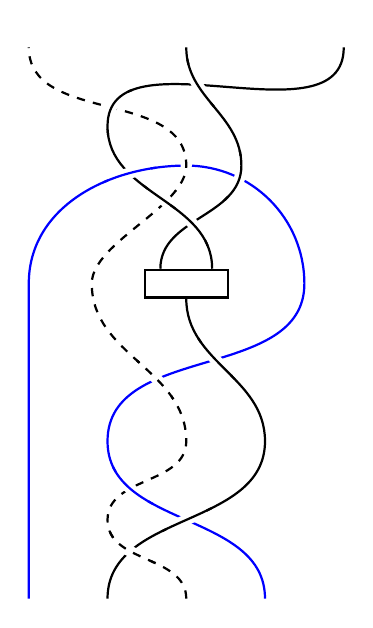
\begin{tikzpicture}
\node (A) at (0,4) [draw,minimum width=30pt,minimum height=10pt,thick] {};
\begin{knot}[
%  draft mode=crossings,
  background colour=white,
  clip width=5,
  clip radius=8pt,
%  consider self intersections,
]
\strand [thick,only when rendering/.style={dashed}] (0,0)
to [out=up, in=down] (-1,1)
to [out=up, in=down] (0,2)
to [out=up, in=down] (-1.2,4)
to [out=up, in=down, looseness=0.7] (0,5.5)
to [out=up, in=down] (-2,7);
\strand [thick] (-1,0)
to [out=up, in=down] (1,2)
to [out=up, in=down] (A.south);
\strand [thick,only when rendering/.style={blue}] (1,0)
to [out=up, in=down] (-1,2)
to [out=up, in=down] (1.5,4)
to [out=up, in=right] (0,5.5)to [out=left, in=up] (-2,4)
to [out=down, in=up] (-2,0);
\strand [thick] (A.150)
to [out=up, in=down] (0.7,5.5)
to [out=up, in=down] (0,7);
\strand [thick] (A.30)
to [out=up, in=down] (-1,6)
to [out=up, in=down] (2,7);
\flipcrossings{6,2,9,5,11}
%\redraw{3}{(0,5.5)}
\end{knot}
\end{tikzpicture}
\end{document}
%% \documentclass{article}
%% \usepackage{tikz}
%% \usepackage{knots}
%% \begin{document}
%% \tikzset{knot/only when rendering/.style={draw=white, double=red}}
%% \newsavebox{\firstbox}
%% \sbox{\firstbox}{\begin{tikzpicture}[remember picture]
%%     \begin{knot}
%%         \strand (1,0) to (0,1);
%%         \strand (0,0) to (1,1);
%%     \end{knot}
%% \end{tikzpicture}}
%% \newsavebox{\secondbox}
%% \sbox{\secondbox}{\begin{tikzpicture}[remember picture]
%%     \node at (0,0) {hello};
%% \end{tikzpicture}}
%% \begin{tikzpicture}
%% \node at (0,0) {\usebox\firstbox};
%% \node at (1,0) {\usebox\secondbox};
%% \end{tikzpicture}
%% \end{document}
\documentclass{article}
\usepackage{nopageno,tikz,knots,geometry}
\geometry{landscape}

\definecolor{SafetyOrange}{rgb}{1,0.4,0}
\definecolor{LuminousOrange}{rgb}{1,0.137255,0.00392157}

\begin{document}

\hspace{-0.75in}
\noindent
\newcommand{\motif}[1]{ 
  to ++(180+#1:0.50) arc (270+#1:150+#1:0.15) 
  to ++( 60+#1:0.50) arc (-30+#1:150+#1:0.15) 
  to ++(240+#1:0.25) arc (150+#1:330+#1:0.25)
  to ++( 60+#1:0.55) arc (150+#1: 30+#1:0.20)
}
\newcommand{\celticknot}{\motif{0}\motif{120}\motif{240}}
\begin{tikzpicture}
\begin{knot}[
  line width=6pt,
  line join=round,
  clip width=1.5,
  clip radius=16pt,
  end tolerance=20pt,
  scale=8,
  consider self intersections,
  ignore endpoint intersections=false,
  background color=red,
  intersection 12/.style={/tikz/knot diagram/clip radius=13pt},
  every strand/.style={draw=none},
  only when rendering/.style={draw=red,double=white,line cap=round,double distance=6pt},
]
\strand (0,0) \celticknot;
\flipcrossings{1,3,6,8,10}
\end{knot}
\end{tikzpicture}

\vfill

\end{document}

\documentclass{article}
\usepackage{tikz,knots}


\newcommand{\motif}[1]{ to ++(180+#1:0.5) arc (270+#1:150+#1:0.15) to ++(60+#1:0.5) arc (-30+#1:150+#1:0.15) to ++(240+#1:0.25) arc (150+#1:330+#1:0.25) to ++(60+#1:0.5) arc (150+#1:30+#1:0.2) }
\newcommand{\celticknot}{\motif{0}\motif{120}\motif{240}}
\begin{document}
\begin{tikzpicture}[line width=3,line join=round,scale=2]
\path[draw=none] (0,0) -- (2,0);
\begin{knot}[
  clip width=1.5pt,
  clip radius=10pt,
  end tolerance=10pt,
%  background colour=red,
  scale=2,
%  draft mode=crossings,
  consider self intersections=no splits,
  ignore endpoint intersections=false,
  draft/crossing label/.style={text opacity=1,text=blue,anchor=south east,append after command={(\tikzlastnode.center) edge[blue,->,thin] (\tikzlastnode.south east)}},
]
\strand[draw=none,only when rendering/.style={draw,double}] (0,0) \celticknot;
\flipcrossings{9,7,5,2,4,11,12}
\end{knot}
\end{tikzpicture}
\end{document}
\begin{tikzpicture}
\begin{knot}[
  consider self intersections,
]
\strand (0,0) .. controls +(2,1) and +(-2,1) .. (1,0);
\end{knot}
\end{tikzpicture}
\end{document}
\documentclass{article}
\usepackage{tikz}
\usepackage{knots}
\begin{document}
\begin{tikzpicture}
\braid[
  rotate=90,
  ultra thick,
  style strands={1}{red},
  style strands={2}{black},
  style strands={3}{blue},
  style strands={4}{green},
] a_1 a_1 a_2^{-1} a_2^{-1} a_1^{-1} a_1^{-1} a_2 a_2 a_2 a_3^{-1} a_3^{-1} a_2^{-1} a_2^{-1} a_2^{-1} a_1 a_1 a_2 a_2 a_1^{-1} a_1^{-1} a_2 a_3 a_3 a_2^{-1};
\end{tikzpicture}
\end{document}
%% \usepackage{tikz}
%% \usepackage{knots}
%% \begin{document}
%% \begin{tikzpicture}
%% \draw (0,0) -- (1,0);
%% \begin{scope}[line width=2pt,scale=2,rotate=45]%,shift={(1cm,2cm)}]
%% \begin{knot}[draft mode=crossings]
%% \strand[red] (0,0) -- (2,2);
%% \strand[blue] (2,0) -- (0,2);
%% \end{knot}
%% \end{scope}
%% \end{tikzpicture}
%% \end{document}



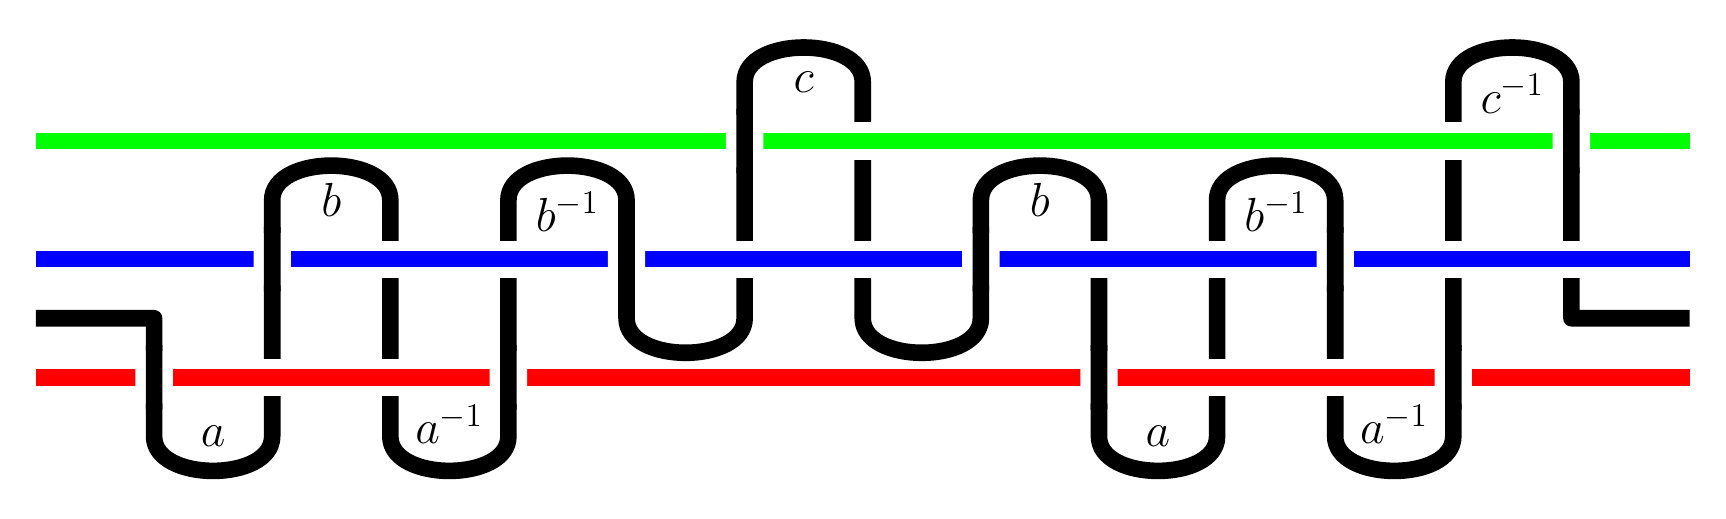
\begin{tikzpicture}[line width=6,line join=round,scale=1.5]
%\def\x{1.5}
%\def\y{1.5}
\def\x{1}
\def\y{1}
\begin{knot}[clip width=1.5]
\strand[red  ] (0*\x,0.0*\y) to (14*\x,0*\y);
\strand[blue ] (0*\x,1.0*\y) to (14*\x,1*\y);
\strand[green] (0*\x,2.0*\y) to (14*\x,2*\y);
\strand[black] (0*\x,0.5*\y) to[out=right,in=left] ++(\x,0)
  to ++(0,-1*\y) to[out=down,in=down] ++(\x,0)
  to ++(0, 2*\y) to[out=up  ,in=up  ] ++(\x,0)
  to ++(0,-2*\y) to[out=down,in=down] ++(\x,0)
  to ++(0, 2*\y) to[out=up  ,in=up  ] ++(\x,0)
  to ++(0,-1*\y) to[out=down,in=down] ++(\x,0)
  to ++(0, 2*\y) to[out=up  ,in=up  ] ++(\x,0)
  to ++(0,-2*\y) to[out=down,in=down] ++(\x,0)
  to ++(0, 1*\y) to[out=up  ,in=up  ] ++(\x,0)
  to ++(0,-2*\y) to[out=down,in=down] ++(\x,0)
  to ++(0, 2*\y) to[out=up  ,in=up  ] ++(\x,0)
  to ++(0,-2*\y) to[out=down,in=down] ++(\x,0)
  to ++(0, 3*\y) to[out=up  ,in=up  ] ++(\x,0)
  to ++(0,-2*\y) to[out=right,in=left] ++(\x,0)
;
\flipcrossings{1,4,5,8,9,12,15,18,21,24}
\end{knot}
\draw
( 1.5*\x,-0.5*\y)     node {\LARGE$a$}
( 2.5*\x, 1.5*\y)     node {\LARGE$b$}
( 3.5*\x,-0.5*\y+0.1) node {\LARGE$a^{-1}$}
( 4.5*\x, 1.5*\y-0.1) node {\LARGE$b^{-1}$}
( 6.5*\x, 2.5*\y)     node {\LARGE$c$}
( 8.5*\x, 1.5*\y)     node {\LARGE$b$}
( 9.5*\x,-0.5*\y)     node {\LARGE$a$}
(10.5*\x, 1.5*\y-0.1) node {\LARGE$b^{-1}$}
(11.5*\x,-0.5*\y+0.1) node {\LARGE$a^{-1}$}
(12.5*\x, 2.5*\y-0.1) node {\LARGE$c^{-1}$}
;
\end{tikzpicture}

\vfill

\end{document}
%\documentclass[border=10]{standalone}
\begin{tikzpicture}
\begin{knot}[draft mode]
\strand[red,ultra thick]  (0,0) .. controls +(1,0) and +(-1,0) .. ++(2,-1) .. controls +(1,0) and +(-1,0) .. ++(2,1) .. controls +(1,0) and +(-1,0) .. ++(2,-1) .. controls +(1,0) and +(-1,0) .. ++(2,1);
\strand[blue,ultra thick] (0,-1) .. controls +(1,0) and +(-1,0) .. ++(2,1) .. controls +(1,0) and +(-1,0) .. ++(2,-1) .. controls +(1,0) and +(-1,0) .. ++(2,1) .. controls +(1,0) and +(-1,0) .. ++(2,-1);
\crossing{1-2-1}{1}
\crossing{1-2-2}{2}
\crossing{1-2-3}{1}
\crossing{1-2-4}{2}
\end{knot}
\end{tikzpicture}

\begin{tikzpicture}
\begin{knot}[draft mode=false]
\strand[red,ultra thick]  (0,0) .. controls +(1,0) and +(-1,0) .. ++(2,-1) .. controls +(1,0) and +(-1,0) .. ++(2,1) .. controls +(1,0) and +(-1,0) .. ++(2,-1) .. controls +(1,0) and +(-1,0) .. ++(2,1);
\strand[blue,ultra thick] (0,-1) .. controls +(1,0) and +(-1,0) .. ++(2,1) .. controls +(1,0) and +(-1,0) .. ++(2,-1) .. controls +(1,0) and +(-1,0) .. ++(2,1) .. controls +(1,0) and +(-1,0) .. ++(2,-1);
\crossing{1-2-1}{1}
\crossing{1-2-2}{2}
\crossing{1-2-3}{1}
\crossing{1-2-4}{2}
\end{knot}
\end{tikzpicture}
\end{document}

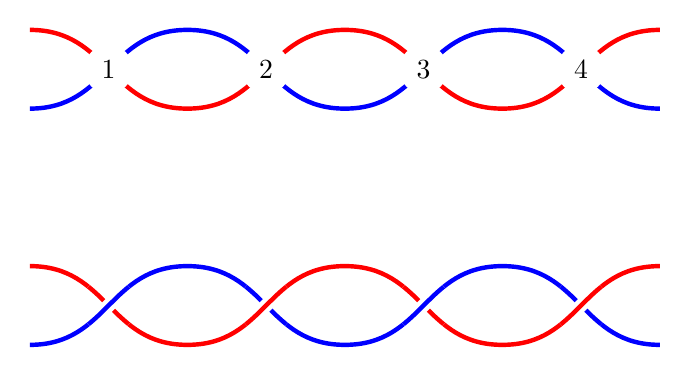
\begin{tikzpicture}
\draw[ultra thick, red,save path=\toppath] (0,0) .. controls +(1,0) and +(-1,0) .. ++(2,-1) .. controls +(1,0) and +(-1,0) .. ++(2,1) .. controls +(1,0) and +(-1,0) .. ++(2,-1) .. controls +(1,0) and +(-1,0) .. ++(2,1);
\draw[ultra thick, blue,save path=\botpath] (0,-1) .. controls +(1,0) and +(-1,0) .. ++(2,1) .. controls +(1,0) and +(-1,0) .. ++(2,-1) .. controls +(1,0) and +(-1,0) .. ++(2,1) .. controls +(1,0) and +(-1,0) .. ++(2,-1);
%\pgfintersectionsortbyfirstpath
\pgfintersectionofpaths{\pgfsetpath\toppath}{\pgfsetpath\botpath}
\foreach \intsect in {1,...,\pgfintersectionsolutions} {
  \pgfpointintersectionsolution{\intsect}
  \pgfgetlastxy{\intsectx}{\intsecty}
  \node[circle,fill=white] at (\intsectx,\intsecty) {\intsect};
}
\begin{scope}[yshift=-3cm]
\draw[ultra thick, red] (0,0) .. controls +(1,0) and +(-1,0) .. ++(2,-1) .. controls +(1,0) and +(-1,0) .. ++(2,1) .. controls +(1,0) and +(-1,0) .. ++(2,-1) .. controls +(1,0) and +(-1,0) .. ++(2,1);
\draw[ultra thick, blue] (0,-1) .. controls +(1,0) and +(-1,0) .. ++(2,1) .. controls +(1,0) and +(-1,0) .. ++(2,-1) .. controls +(1,0) and +(-1,0) .. ++(2,1) .. controls +(1,0) and +(-1,0) .. ++(2,-1);
\foreach \intsect in {1,...,\pgfintersectionsolutions} {
  \begin{scope}
  \pgfpointintersectionsolution{\intsect}
  \pgfgetlastxy{\intsectx}{\intsecty}
  \clip  (\intsectx,\intsecty) circle[radius=10pt];
\ifodd\intsect
\draw[ultra thick,double=red,double distance=1.6pt,white] (0,0) .. controls +(1,0) and +(-1,0) .. ++(2,-1) .. controls +(1,0) and +(-1,0) .. ++(2,1) .. controls +(1,0) and +(-1,0) .. ++(2,-1) .. controls +(1,0) and +(-1,0) .. ++(2,1);
\fi
\draw[ultra thick,double=blue,double distance=1.6pt,white] (0,-1) .. controls +(1,0) and +(-1,0) .. ++(2,1) .. controls +(1,0) and +(-1,0) .. ++(2,-1) .. controls +(1,0) and +(-1,0) .. ++(2,1) .. controls +(1,0) and +(-1,0) .. ++(2,-1);
\ifodd\intsect
\else
\draw[ultra thick,double=red,double distance=1.6pt,white] (0,0) .. controls +(1,0) and +(-1,0) .. ++(2,-1) .. controls +(1,0) and +(-1,0) .. ++(2,1) .. controls +(1,0) and +(-1,0) .. ++(2,-1) .. controls +(1,0) and +(-1,0) .. ++(2,1);
\fi
\end{scope}
}
\end{scope}
\end{tikzpicture}
\end{document}

\documentclass{article}
\usepackage{tikz}
\usetikzlibrary{intersections}
\usepackage{spath}

\makeatletter
\def\splitcurveto#1#2\pgfsyssoftpath@curvetosupportatoken#3#4\pgfsyssoftpath@curvetosupportbtoken#5#6\pgfsyssoftpath@curvetotoken#7#8{%
  \pgfmathsetmacro{\knot@ax}{#1/28}
  \pgfmathsetmacro{\knot@bx}{#3/28}
  \pgfmathsetmacro{\knot@cx}{#5/28}
  \pgfmathsetmacro{\knot@dx}{#7/28}
  \pgfmathsetmacro{\knot@ay}{#2/28}
  \pgfmathsetmacro{\knot@by}{#4/28}
  \pgfmathsetmacro{\knot@cy}{#6/28}
  \pgfmathsetmacro{\knot@dy}{#8/28}
  \message{Got (\knot@ax,\knot@ay), (\knot@bx,\knot@by), (\knot@cx,\knot@cy), (\knot@cx,\knot@cy)}
  \pgfmathsetmacro{\splittimenum}{%
    ( (\knot@ay - 3 * \knot@by + 3 * \knot@cy - \knot@dy) * (3 * \knot@cx - 3 * \knot@dx)
    - (\knot@ax - 3 * \knot@bx + 3 * \knot@cx - \knot@dx) * (3 * \knot@cy - 3 * \knot@dy) )}
  \pgfmathsetmacro{\splittimeden}{%
    ( (\knot@ax - 3 * \knot@bx + 3 * \knot@cx - \knot@dx) * (3 * \knot@by - 6 * \knot@cy + 3 * \knot@dy)
    - (\knot@ay - 3 * \knot@by + 3 * \knot@cy - \knot@dy) * (3 * \knot@bx - 6 * \knot@cx + 3 * \knot@dx) )}
  \pgfmathsetmacro{\splittime}{.5*\splittimenum/\splittimeden}
  \pgfpointcurveattime{\splittime}{\pgfqpoint{#1}{#2}}{\pgfqpoint{#3}{#4}}{\pgfqpoint{#5}{#6}}{\pgfqpoint{#7}{#8}}
  \global\pgf@xa=\pgf@x
  \global\pgf@ya=\pgf@y
}
\def\splitit{\message{split it}}
\def\nosplitit{\message{don't split it}}
\makeatother

\begin{document}
\begin{tikzpicture}
\makeatletter
\draw[save path=\tmppath] (0,0) .. controls +(3,3) and +(2,-2) .. (0,1);
\draw[save path=\tmppath] (0,0) .. controls (2,1) and (-1,1) .. (1,0);
\begingroup
\let\pgfsyssoftpath@movetotoken=\splitcurveto
\tmppath
\endgroup
\fill (\the\pgf@xa,\the\pgf@ya) circle[radius=2pt];
\makeatother

\end{tikzpicture}
\end{document}
\begin{tikzpicture}
\makeatletter
\foreach \k in {0,...,-10} {
\begin{scope}[yshift=\k cm]
\draw[save path=\tmppath] (0,0) .. controls +(3,3) and +(2,-2) .. (\k,1);
\draw[red] (0,0) -- (3,3) -- (\k + 2,-1) -- (\k,1);
\begingroup
\let\pgfsyssoftpath@movetotoken=\splitcurveto
\tmppath
\endgroup
\end{scope}
\fill (\the\pgf@xa,\the\pgf@ya) circle[radius=2pt];
}
\makeatother



\end{tikzpicture}
\end{document}
\draw[save path=\tmppath] (0,0) -- (1,1) .. controls +(1,1) and +(1,-1) .. (1,0) -- (0,1);
\pgfintersectionofpaths{\pgfsetpath\tmppath}{\pgfsetpath\tmppath}
\foreach \ints in {1,...,\pgfintersectionsolutions} {
      \pgfpointintersectionsolution{\ints}
      \pgfgetlastxy{\intsectx}{\intsecty}
  \fill (\intsectx,\intsecty) circle[radius=2pt];
}
\end{tikzpicture}
\end{document}


% Local Variables:
% tex-output-type: "pdf18"
% End:
